\documentclass[tikz,border=6pt]{standalone}

\usepackage[T1]{fontenc}
\usepackage{lmodern}
\usetikzlibrary{calc}

\begin{document}
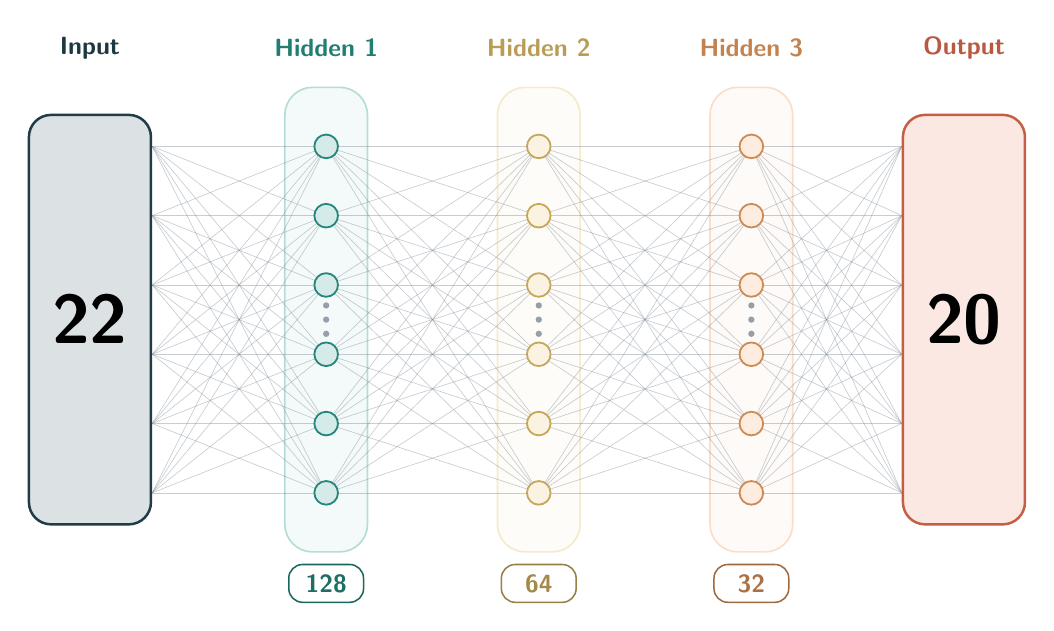
\begin{tikzpicture}[
    x=1cm,
    y=1cm,
    line cap=round,
    line join=round,
    font=\sffamily
]

\definecolor{DeepTeal}{HTML}{264653}
\definecolor{MineralGreen}{HTML}{2A9D8F}
\definecolor{MutedAmber}{HTML}{E9C46A}
\definecolor{WarmSand}{HTML}{F4A261}
\definecolor{CoralRust}{HTML}{E76F51}
\definecolor{LineGray}{HTML}{7B8794}

\tikzset{
    layer block/.style={
        rounded corners=8pt,
        draw=#1!85!black,
        fill=#1!16,
        line width=0.9pt,
        minimum width=1.55cm,
        minimum height=5.2cm,
        inner sep=0pt
    },
    layer frame/.style={
        rounded corners=10pt,
        draw=#1!35,
        fill=#1!5,
        line width=0.6pt,
        minimum width=1.05cm,
        minimum height=5.9cm,
        inner sep=0pt
    },
    neuron/.style={
        circle,
        draw=#1!85!black,
        fill=#1!20,
        line width=0.65pt,
        minimum size=0.30cm,
        inner sep=0pt
    },
    count label/.style={
        rounded corners=5pt,
        draw=#1!65!black,
        fill=white,
        line width=0.55pt,
        minimum width=0.95cm,
        minimum height=0.48cm,
        inner sep=2pt,
        text=#1!70!black,
        font=\sffamily\bfseries\small
    },
    stage label/.style={
        text=#1!80!black,
        font=\sffamily\bfseries\small
    },
    connector/.style={
        draw=LineGray,
        line width=0.24pt,
        opacity=0.42
    },
    dot/.style={
        circle,
        fill=LineGray!80,
        draw=none,
        minimum size=0.08cm,
        inner sep=0pt
    }
}

\node[layer block=DeepTeal] (input) at (0,0) {\fontsize{24}{24}\selectfont\bfseries 22};
\node[layer block=CoralRust] (output) at (11.1,0) {\fontsize{24}{24}\selectfont\bfseries 20};

\node[layer frame=MineralGreen] at (3.0,0) {};
\node[layer frame=MutedAmber] at (5.7,0) {};
\node[layer frame=WarmSand] at (8.4,0) {};

\node[stage label=DeepTeal] at (0,3.45) {Input};
\node[stage label=MineralGreen] at (3.0,3.45) {Hidden 1};
\node[stage label=MutedAmber] at (5.7,3.45) {Hidden 2};
\node[stage label=WarmSand] at (8.4,3.45) {Hidden 3};
\node[stage label=CoralRust] at (11.1,3.45) {Output};

\foreach \y/\name in {2.20/h11,1.32/h12,0.44/h13,-0.44/h14,-1.32/h15,-2.20/h16} {
    \node[neuron=MineralGreen] (\name) at (3.0,\y) {};
}
\foreach \y/\name in {2.20/h21,1.32/h22,0.44/h23,-0.44/h24,-1.32/h25,-2.20/h26} {
    \node[neuron=MutedAmber] (\name) at (5.7,\y) {};
}
\foreach \y/\name in {2.20/h31,1.32/h32,0.44/h33,-0.44/h34,-1.32/h35,-2.20/h36} {
    \node[neuron=WarmSand] (\name) at (8.4,\y) {};
}

\foreach \x in {3.0,5.7,8.4} {
    \foreach \y in {0.18,0.0,-0.18} {
        \node[dot] at (\x,\y) {};
    }
}

\node[count label=MineralGreen] at (3.0,-3.35) {128};
\node[count label=MutedAmber] at (5.7,-3.35) {64};
\node[count label=WarmSand] at (8.4,-3.35) {32};

\foreach \y/\name in {2.20/in1,1.32/in2,0.44/in3,-0.44/in4,-1.32/in5,-2.20/in6} {
    \coordinate (\name) at ($(input.east)+(0,\y)$);
}
\foreach \y/\name in {2.20/out1,1.32/out2,0.44/out3,-0.44/out4,-1.32/out5,-2.20/out6} {
    \coordinate (\name) at ($(output.west)+(0,\y)$);
}

\foreach \i in {1,...,6} {
    \foreach \j in {1,...,6} {
        \draw[connector] (in\i) -- (h1\j);
        \draw[connector] (h1\i) -- (h2\j);
        \draw[connector] (h2\i) -- (h3\j);
        \draw[connector] (h3\i) -- (out\j);
    }
}

\end{tikzpicture}
\end{document}